\begin{figure}[p]\centering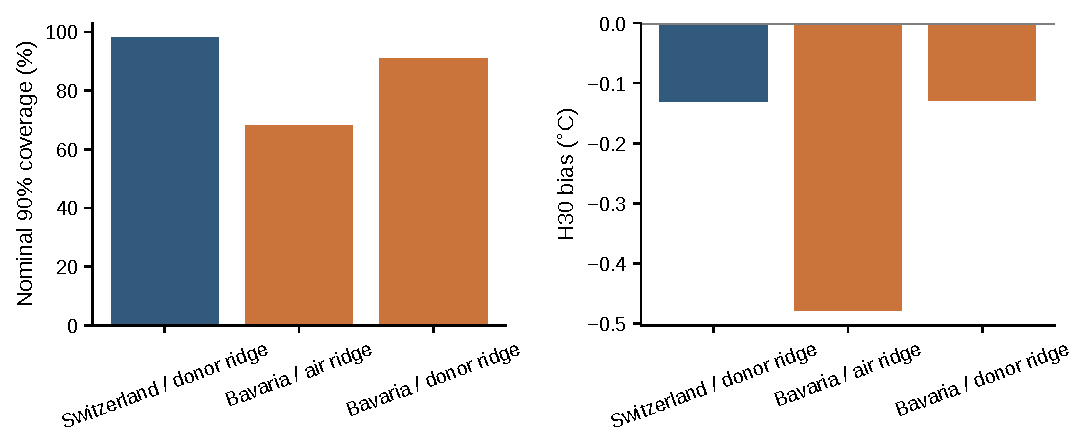
\includegraphics[width=\textwidth]{figures/process_revision/02_region_recovery.pdf}\caption{Hidden-reference-peak recovery by region and daily reconstructor. Coverage is nominal 90\%; bias is the median minus complete-year H30. The hidden-peak label uses withheld complete-year truth and is unavailable at decision time. Bavarian air-ridge cases are not matched to Swiss donor-ridge cases.}\label{fig:region-recovery}\end{figure}
\begin{figure}[p]\centering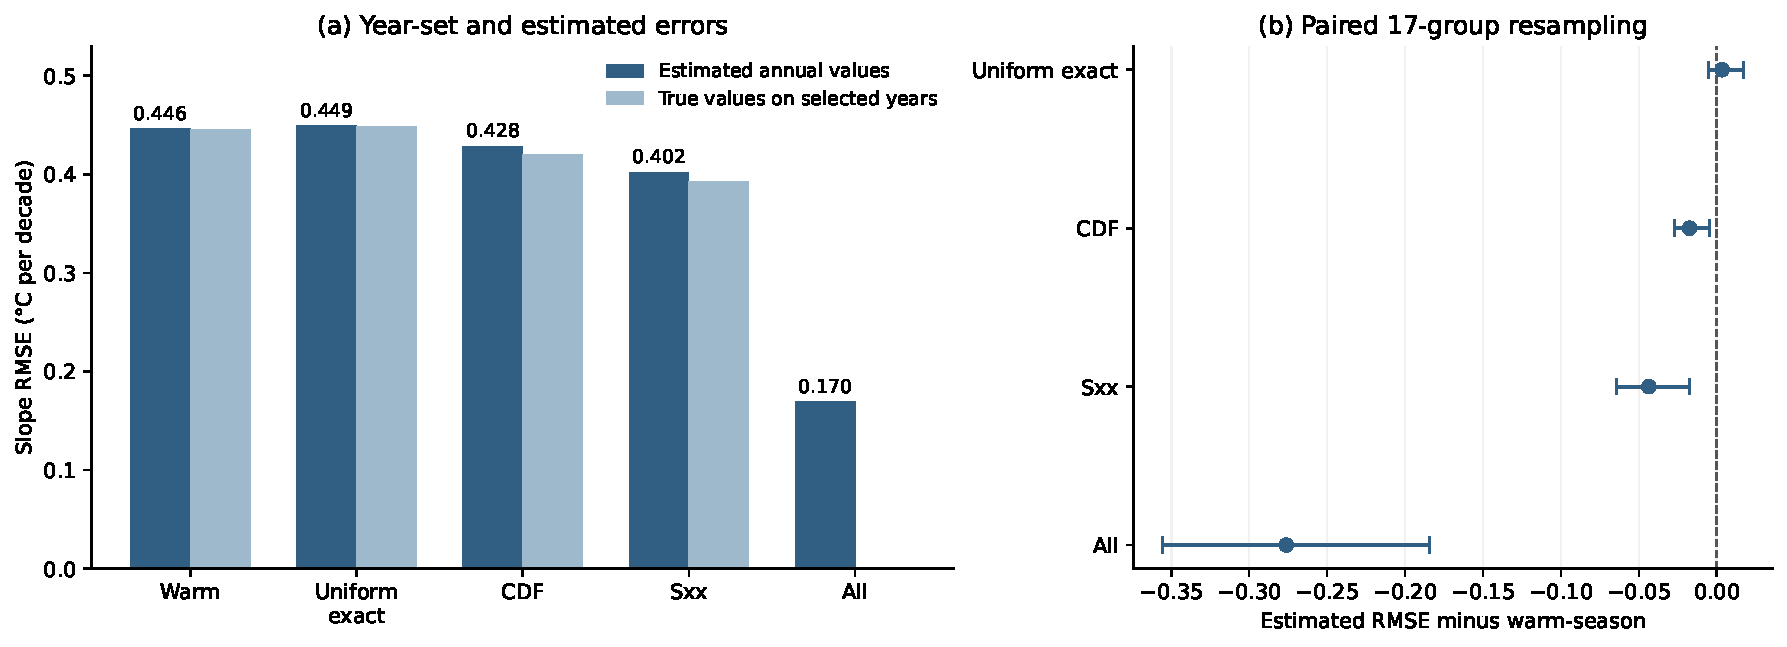
\includegraphics[width=\textwidth]{figures/process_revision/03_time_support.pdf}\caption{Year choice at a fixed retention count on 805 forward controlled-gap archives. Left: estimated-slope and complete-truth-year-set RMSE. Uniform exact averages squared error over every feasible subset inside each archive before taking the cohort root. CDF and $S_{xx}$ select years without temperature outcomes and include all fixed complete years in their objectives. Right: comparator-minus-warm-season estimated-RMSE differences and paired 95\% percentile intervals from 10,000 resamples of 17 connected groups. The original one-draw random and incomplete-year-only spacing controls remain in Table~\ref{tab:time-support}.}\label{fig:time-support}\end{figure}
\begin{figure}[p]\centering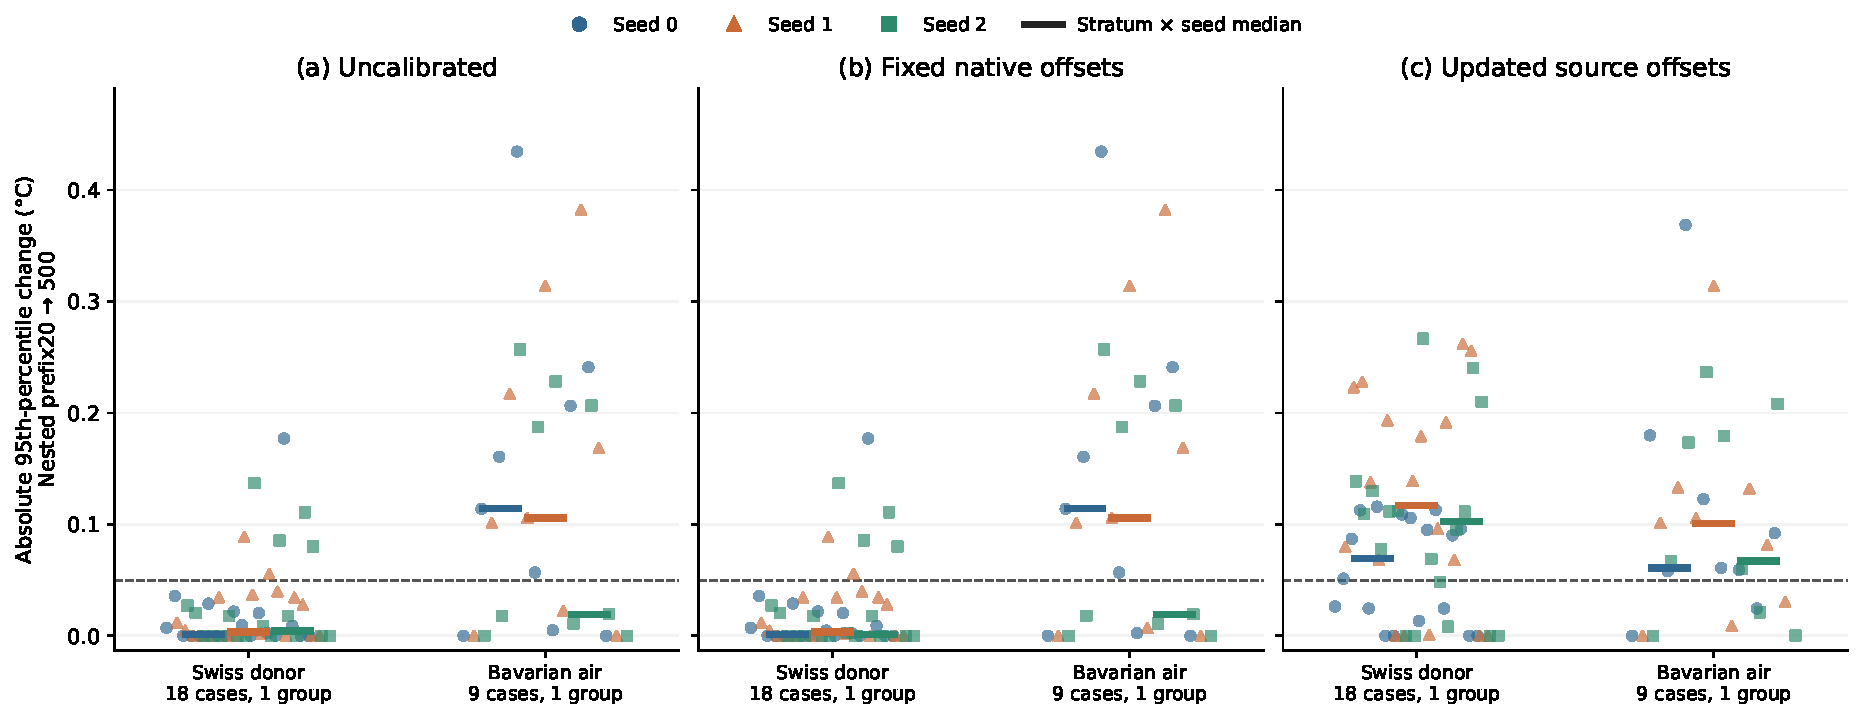
\includegraphics[width=\textwidth]{figures/process_revision/04_trajectory_budget.pdf}\caption{Absolute upper-endpoint changes between nested 20 and 500 residual-bridge paths, for the same target samples under no offset, fixed historical source offsets and source offsets re-estimated at each budget. All 27 case points per seed remain visible, separated into 18 Swiss donor-ridge and nine Bavarian air-ridge cases; colors identify seeds 0, 1 and 2 and horizontal marks their stratum medians. The 0.05$^{\circ}$C line is a numerical diagnostic. Source recalibration uses 2,370 original positive-weight cases with unchanged roles and multiplicities. Native historical 20-path draws are a separate reference, not the 500-path prefix. Lower-endpoint changes and all counts are reported in Supporting Information. Two target groups and 500 paths do not establish population calibration or convergence.}\label{fig:trajectory-budget}\end{figure}
